% Standalone render of generated_intraday/table_rule_by_strategy_intraday_1500.tex
% Build: pdflatex -interaction=nonstopmode rule_by_strategy_intraday_1500.tex
\documentclass{article}
\usepackage[landscape,margin=0.5in]{geometry}
\usepackage{booktabs}
\usepackage{amsmath}
\usepackage{graphicx}
\pagestyle{empty}

\begin{document}
\begin{center}
\textbf{0DTE nearest-OTM package: per-rule return summary, entry 15:00 ET, one-bar hold, models compared on the same 866 days}\\[1.5ex]
% AUTO-GENERATED by writeup/make_rule_by_strategy_intraday_tex.py -- do not edit.
% Source: results/atm_straddle_intraday/rule_by_strategy/1500/rule_by_strategy_*.csv
\begingroup\small\setlength{\tabcolsep}{3.6pt}
\begin{tabular}{lrrrrrrrrrrrr}
\toprule
& $n$ & mean & std & min & max & skew & ex.\ kurt & $t$ & Sharpe$_{\mathrm{clk}}$ & $n_{\mathrm{buy}}$ & \%buy & Sharpe$^{\times}_{\mathrm{clk}}$ \\
\midrule
\multicolumn{13}{l}{\emph{Short volatility (always short)}} \\
all models (no forecast) & 866 & 0.060 & 0.379 & -3.31 & 0.58 & -3.03 & 15.14 & 4.64 & 2.51 & 0 & 0.0 & 0.18 \\
\midrule
\multicolumn{13}{l}{\emph{$\mathrm{sign}(s)$ ($\pm 1$ on the sign of $s$)}} \\
baseline (HAR + calendar OLS) & 866 & 0.026 & 0.383 & -3.31 & 2.85 & -1.16 & 13.02 & 2.01 & 1.08 & 201 & 23.2 & -1.20 \\
block-diagonal ridge & 866 & 0.033 & 0.383 & -3.31 & 2.85 & -0.97 & 13.11 & 2.52 & 1.36 & 186 & 21.5 & -0.93 \\
block-diagonal ridge, without the FOMC columns & 866 & 0.032 & 0.383 & -3.31 & 2.85 & -0.96 & 13.08 & 2.45 & 1.32 & 189 & 21.8 & -0.97 \\
LightGBM$^{\dagger}$ & 866 & 0.024 & 0.383 & -3.31 & 2.85 & -1.08 & 12.96 & 1.86 & 1.00 & 205 & 23.7 & -1.28 \\
XGBoost$^{\dagger}$ & 866 & 0.022 & 0.383 & -3.31 & 2.85 & -1.07 & 12.92 & 1.69 & 0.91 & 220 & 25.4 & -1.37 \\
lasso (causally tuned)$^{\dagger}$ & 866 & 0.033 & 0.382 & -3.31 & 2.85 & -0.84 & 13.07 & 2.55 & 1.37 & 198 & 22.9 & -0.92 \\
lasso ($\alpha=10^{-4}$) & 866 & 0.034 & 0.382 & -3.31 & 2.85 & -0.97 & 13.13 & 2.61 & 1.41 & 185 & 21.4 & -0.89 \\
elastic net (causally tuned)$^{\dagger}$ & 866 & 0.029 & 0.383 & -3.31 & 2.85 & -1.19 & 13.09 & 2.22 & 1.20 & 190 & 21.9 & -1.09 \\
\bottomrule
\end{tabular}
\endgroup

\end{center}
\vspace{1ex}
\begin{center}
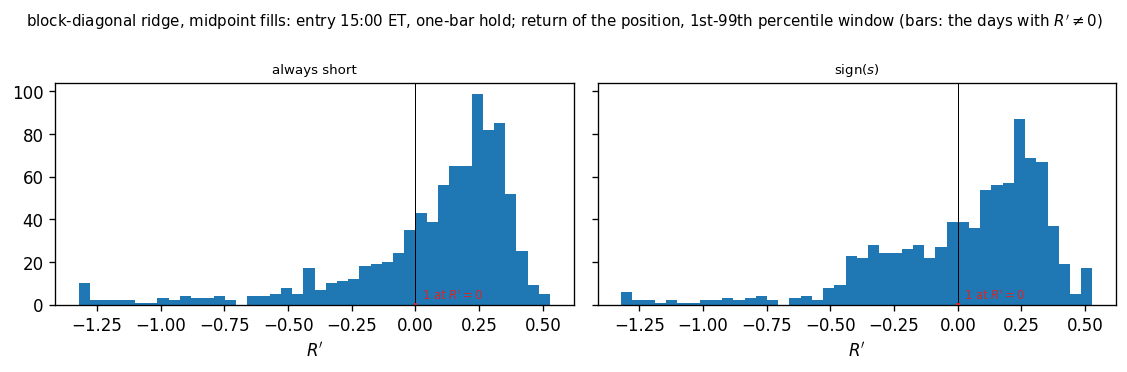
\includegraphics[width=0.52\textwidth]{../results/atm_straddle_intraday/rule_by_strategy/1500/rule_hists_blk2_1500.png}\par\smallskip
\small Distribution of the return of the position taken at 15:00 ET, block-diagonal ridge forecast, one panel per rule (returns inside their 1st--99th percentile window).
\end{center}
\vspace{1ex}
\noindent\small One trade a day: enter the nearest-OTM package at 15:00 ET and exit thirty minutes later at the next stamp, in the same two strikes. 866 expiration days, 2020-01-03 to 2024-04-30 (the deck's frame). Fills are at the quoted midpoint everywhere except the last column, which is the same rule filled at the crossed spread: entry at the touch (the ask when long, the bid when short) and exit at the touch of the next stamp; the 15:30 leg cash-settles and pays no exit spread, and a re-pick that lands on the same two strikes with the same sign is a hold, not a round trip, so it is not charged.
\vspace{1ex}
\noindent\small One expiration day = one return; mid fill. Every $t$ here is the plain
$t=\sqrt{n}\cdot\mathrm{mean}/\mathrm{std}$, with no autocorrelation correction.
``ex.\ kurt'' is the bias-corrected sample excess kurtosis (Gaussian $=0$).
The short-volatility rule takes no forecast, so it is one row for all models.
\textbf{Two Sharpes.} Both multiply by $\sqrt{252}$ because an expiration day is
the unit of time (same year-length as the paper). They are not the same object.
On a \emph{single-clock} page, Sharpe$_{\mathrm{clk}}=(\mathrm{mean}/\mathrm{std})\times\sqrt{252}$
of that clock's series: one 30-minute hold per expiration day. It answers ``if I
only entered at this clock, what is my annual Sharpe?'' It is \emph{not} the
book's Sharpe$_{\mathrm{ann}}$.
On the \emph{pooled} page, Sharpe$_{\mathrm{ann}}=(\mathrm{mean}/\mathrm{std})\times\sqrt{252}$
of $R^{day}_d=\sum_t R'_{d,t}$, the sum of the day's twelve holds. That reserved
name is the book's daily P\&L after pooling the session. At 15:30 the two
coincide (one trade that day); they do not on 10:00--15:00 or on the pooled page.
Sharpe$^{\times}$ is the same convention at the crossed spread. Every other column is daily.
$n_{\mathrm{buy}}$ is the number of expiration days with position $>0$ (always-short is 0;
on the pooled page it is days the sum of the twelve positions is positive);
\%buy is $100\cdot n_{\mathrm{buy}}/n$, the notebook's column.
The other column this table adds to the deck's is Sharpe$^{\times}_{\mathrm{ann}}$, the same
rule's annualized Sharpe at the \emph{crossed spread} instead of the midpoint; every other
column is the deck's.

\smallskip
\noindent\small Forecasts: baseline (HAR + calendar OLS); block-diagonal ridge (HAR block and exogenous block, separate penalties)
on the design carrying the FOMC calendar block, and the same ridge on the earlier design without those columns, as a diagnostic row;
LightGBM and XGBoost on the all-features design; lasso on the same design, causally tuned vs.\ fixed $\alpha=10^{-4}$;
elastic net (causally tuned). $\dagger$ marks a column still fitted on the earlier design panel; a run of those four on the
panel of record is pending.
The signal is $s_t=\widehat{RV}_t-\mathrm{IV}^{2}_{\mathrm{hr}}h_t w_t$: the forecast against the
implied variance of the same window. $w_t$ is the expanding mean of each prior day's
remaining-session share of realized variance, $\mathrm{RV}_t/\sum_{s\ge t}\mathrm{RV}_s$
(in-fit panel history back to 2001), not the ratio of trailing clock-means.
On the bars whose vendor implied volatility is a censored
solver node the deck's treatment is used here too --- the volatility that reproduces the package
midpoint, recovered by bisection over the remaining $h_t$ hours --- so every bar carries a
signal and no bar sits flat.
\end{document}
